\chapter{Conclusões}
\label{chap6}
 \section{Resultados}
1-2 parag

Com a implentação do sistema admins usuarios interagiram de maneira mais rapida, algun dado, produtividade, retorno pessoal

curto periodo de aprendizado 

\begin{figure}
    \centering
    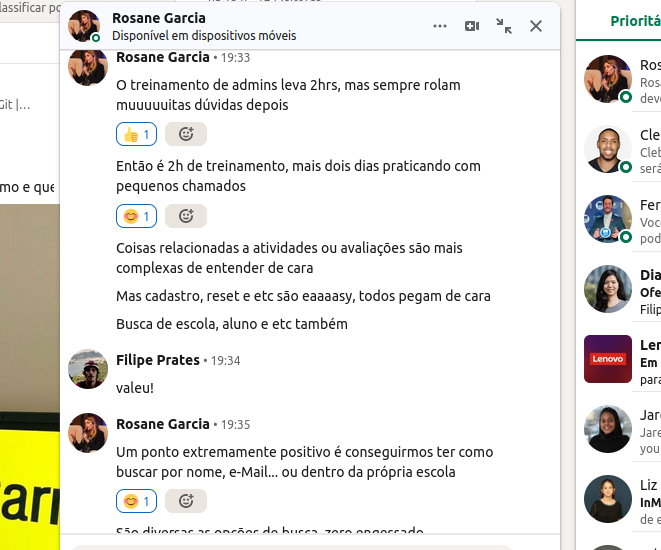
\includegraphics[width=1\linewidth]{image.png}
    \caption{PLACEHOLDER }
    \label{fig:enter-label}
\end{figure}

são diversas opções de busca gero engessado - devido à natureza do grafo, sempre tem diversas maneiras de alcançar um mesmo objetivo (conectar por um lado ou pelo outro, pesquisar em mais de um lugar, e etc)

 \section{Trabalhos Futuros}

Dentre as possíveis implementações adicionais podemos citar:
\begin{itemize}
    \item Apesar de medidas de segurança para garantir que apenas usuários autorizados  ainda é interessante tornar o sistema mais robusto com medidas adicionais de prevenção de acesso à base de dados por usuários de perfil inadequado
- sistema mais robusto
    \item Gerar automaticamente os arquivos que definem as requisições .gql com as informações retornadas pela InstrospectionQuery. A configuração prévia da estrutura de arquivos pode ser um ponto de dor para o desenvolvimento ~
    \item Desenvolver um sistema de interface 'perfil e listas' de maneira compatível à disponibilizar no Neo4j Developer Graph Apps 
\end{itemize}



